\section{Introduction}
Ce projet de pilotage de projet DevOps a pour but de mettre en pratique les connaissances acquises lors du cours avec l'utilisation de Docker et la mise en place de plusieurs services. 2 exercices seront proposés dans ce rendu, à savoir les exercices VIII et IX.
Toutes les justifications sont présentes dans la partie \ref{sec:Annexes}, mais vous pouvez retrouver toutes les sources dans \href{https://github.com/RemiSaurel/docker-homework}{\textbf{ce repository GitHub que j'ai créé}}.

\section{Architecture}
\subsection{Exercice VIII}
\subsubsection*{Architecture générale}
La figure \ref{fig:exo8} présente l'architecture générale de cet exercice. On y retrouve un fichier \verb|docker-compose.yml| qui permet de lancer les 2 services : \verb|app| et \verb|db8|. Le service \verb|app| est le projet Spring Boot fourni. Le service \verb|db8| est une base de données MySQL.

\subsubsection*{Types de réseaux}
Le réseau utilisé est le réseau \verb|bridge| de Docker. Il permet de créer un réseau privé pour les conteneurs. Les ports 3306 et 8080 sont exposés pour pouvoir accéder à la base de données et à l'application Spring Boot.
\subsubsection*{Types de stockages}
Le stockage utilisé est le stockage \verb|volume| de Docker, ici nommé \verb|db_data|. Il permet de créer un volume pour les conteneurs. Il est utilisé pour la base de données afin de pouvoir conserver les données même si le conteneur est supprimé.

\subsection{Exercice IX}
\subsubsection*{Architecture générale}
La figure \ref{fig:exo9} présente l'architecture générale de cet exercice. On y retrouve un fichier \verb|docker-compose.yml| qui permet de lancer les 4 services : \verb|app| et \verb|db|. Le service \verb|app| est le projet Spring Boot fourni. Le service \verb|db| est une base de données MySQL. Le service phpMyAdmin est un service permettant d'interagir avec la base de données. Le service \verb|Sonarqube| est un service permettant d'analyser le code source.
\subsubsection*{Types de réseaux}
Le réseau utilisé est le réseau \verb|bridge| de Docker. Un réseau a été explicitement créé (le réseau `exo9') dans le docker compose et permet aux différents services d'intéragir entre eux. Les ports 3306, 8080 et 9000 sont exposés pour pouvoir accéder à la base de données, à l'application Spring Boot et à Sonarqube.
\subsubsection*{Types de stockages}
Comme pour l'exercice VIII, le stockage utilisé est le stockage \verb|volume| de Docker, ici nommé \verb|db_data|. Il est utilisé pour la base de données afin de pouvoir conserver les données même si le conteneur est supprimé.
\section{Conclusion}
Ce projet m'a permis de mettre en pratique de façon concrète les éléments vus en cours. Cela m'a notamment servi afin de mieux comprendre les notions de volumes et de réseaux qui restaient assez floues. Pour conclure, cela m'a aidé à découvrir comment Docker pouvait être mis en place très facilement ainsi que les différents services qui pouvaient être utilisés.
\newpage

\section{Annexes}\label{sec:Annexes}
Vous pouvez retrouver toutes les sources sur le \href{https://github.com/RemiSaurel/docker-homework}{repository GitHub} que j'ai créé.

\subsection*{Exercice VIII}

\begin{figure}[hbtp]
    \centering
    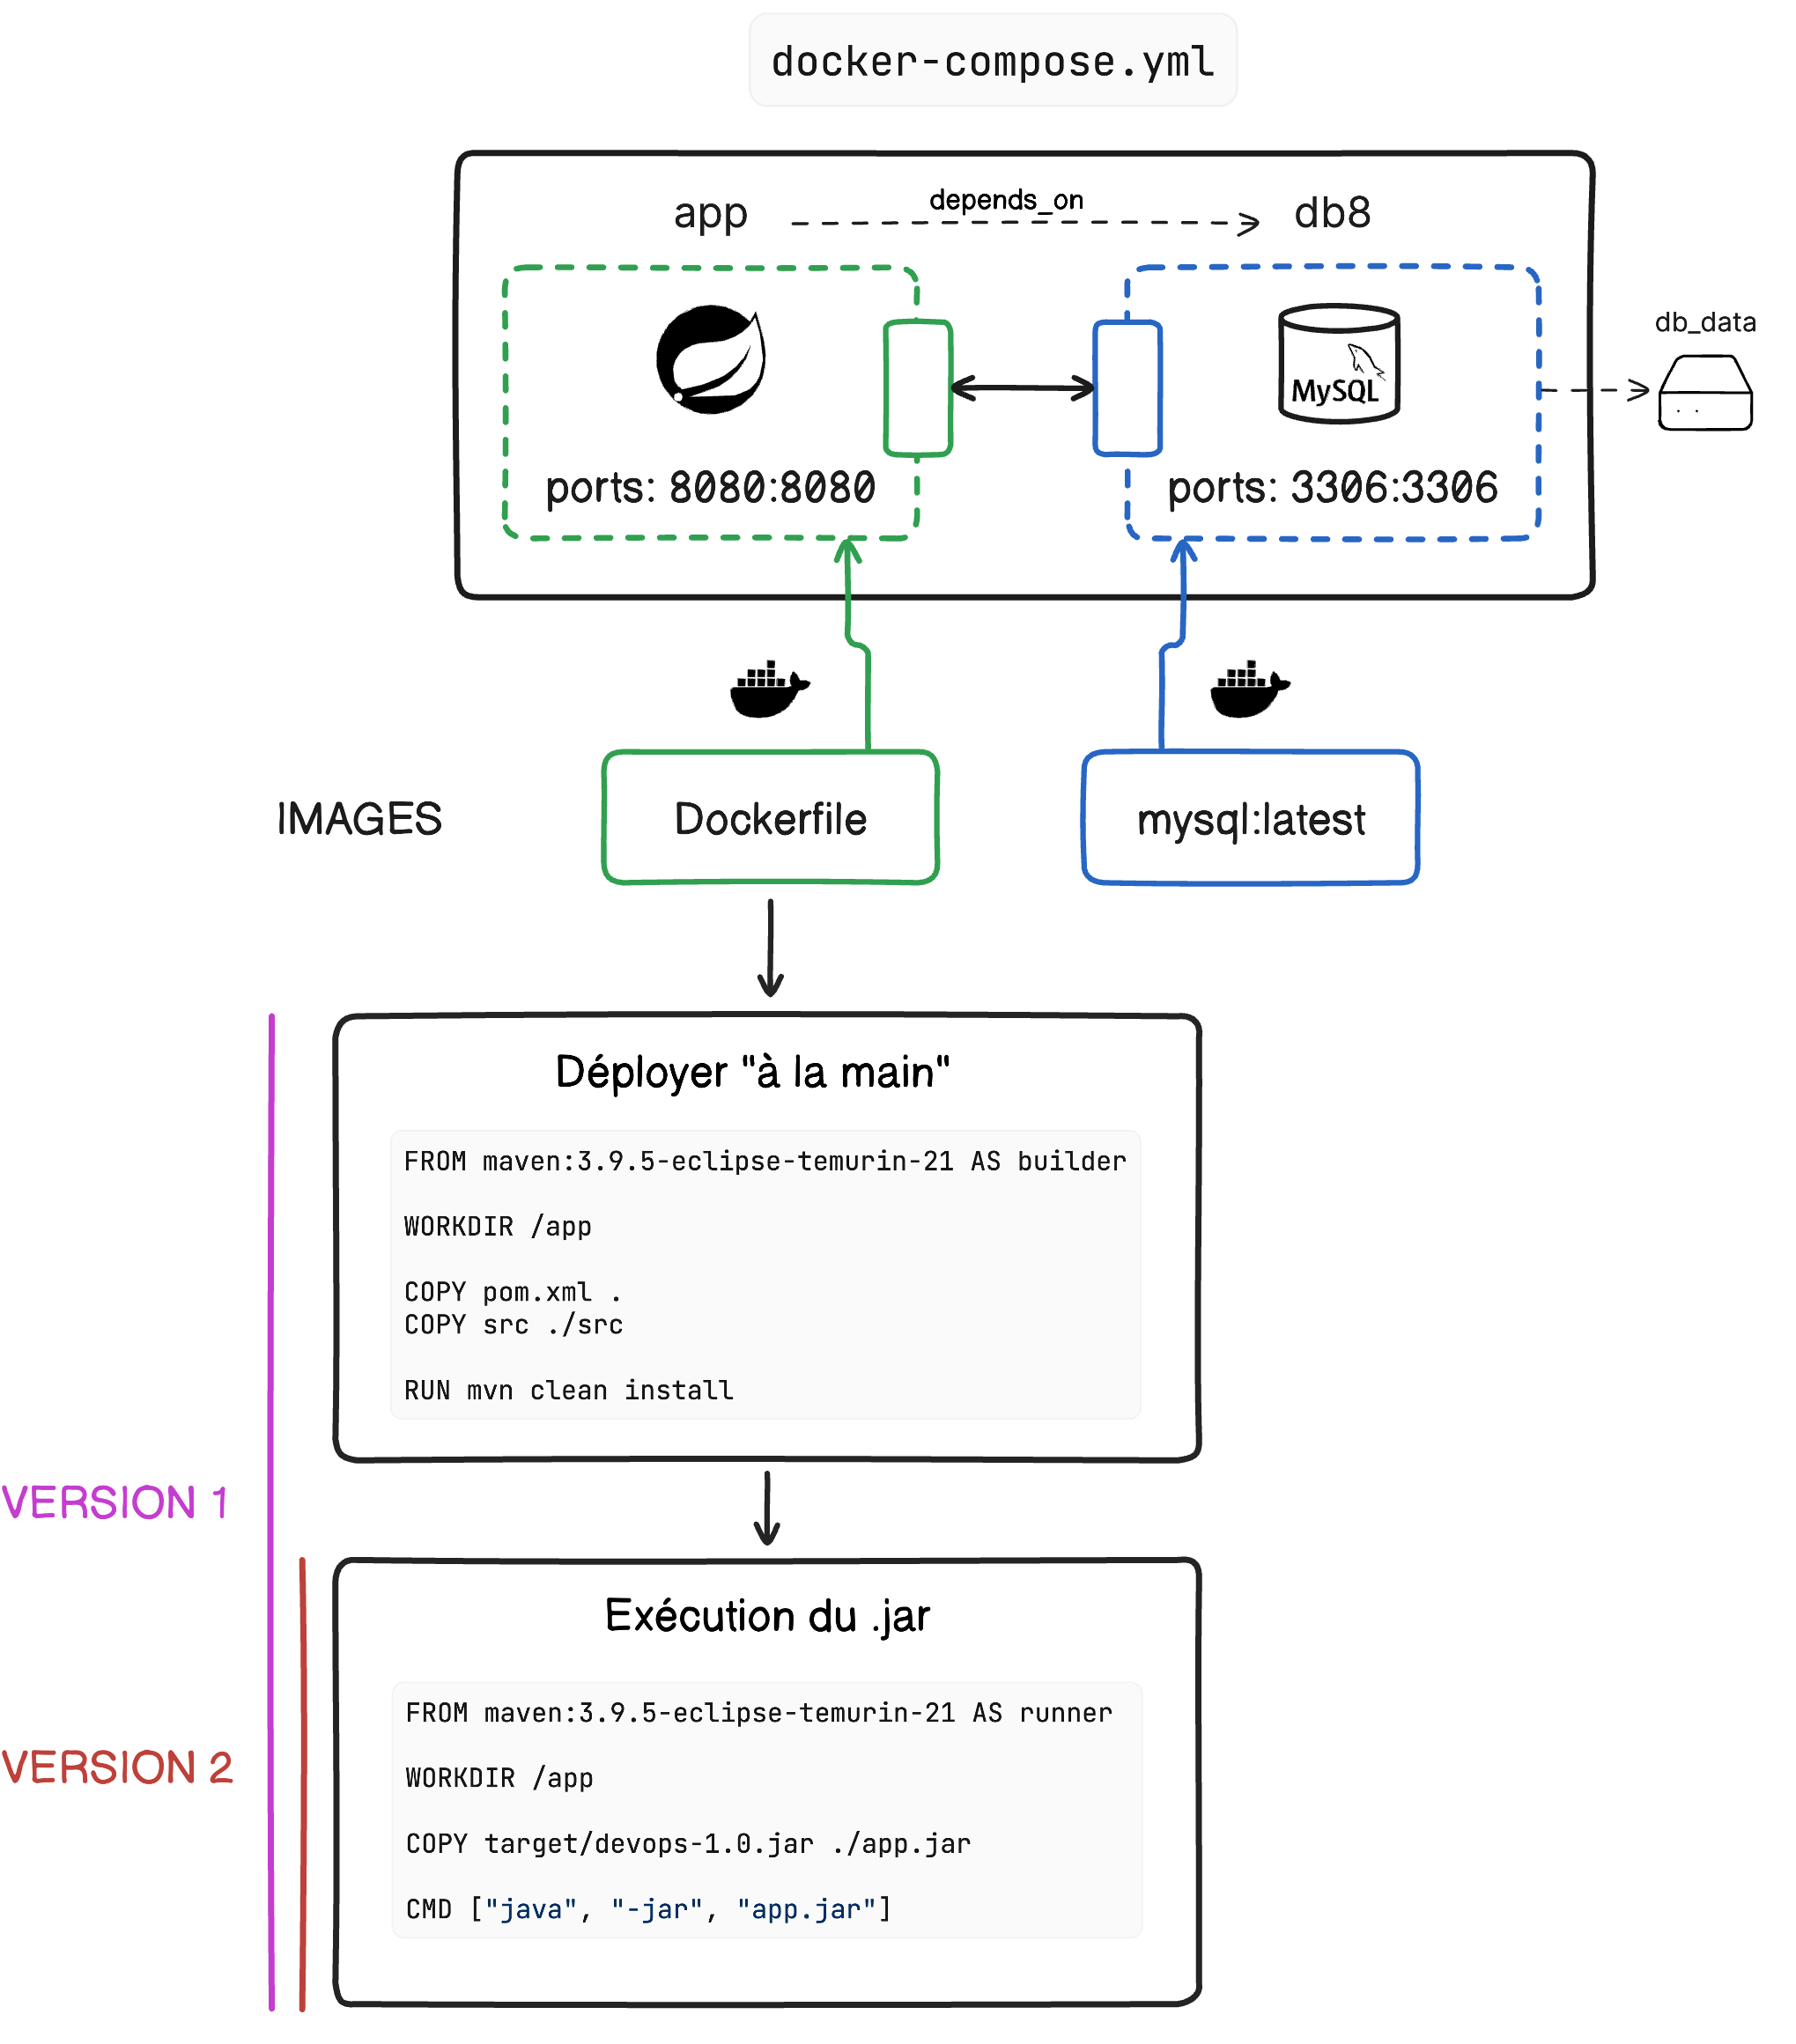
\includegraphics[width=\textwidth]{images/exo8.png}
    \caption{Architecture générale de l'exercice VIII}
    \label{fig:exo8}
\end{figure}

\subsubsection*{Commandes}
Commandes à réaliser :
Dans le fichier Dockerfile, commenter / décommenter les lignes
pour build ou non l'application Spring Boot.
    
\begin{verbatim}
    docker compose up -d
\end{verbatim}
Pour arrêter et supprimer les containers, vous pouvez utiliser :

\begin{verbatim}
    docker compose down
\end{verbatim}

\subsubsection*{Résultats}

\begin{figure}[hbtp]
    \centering
    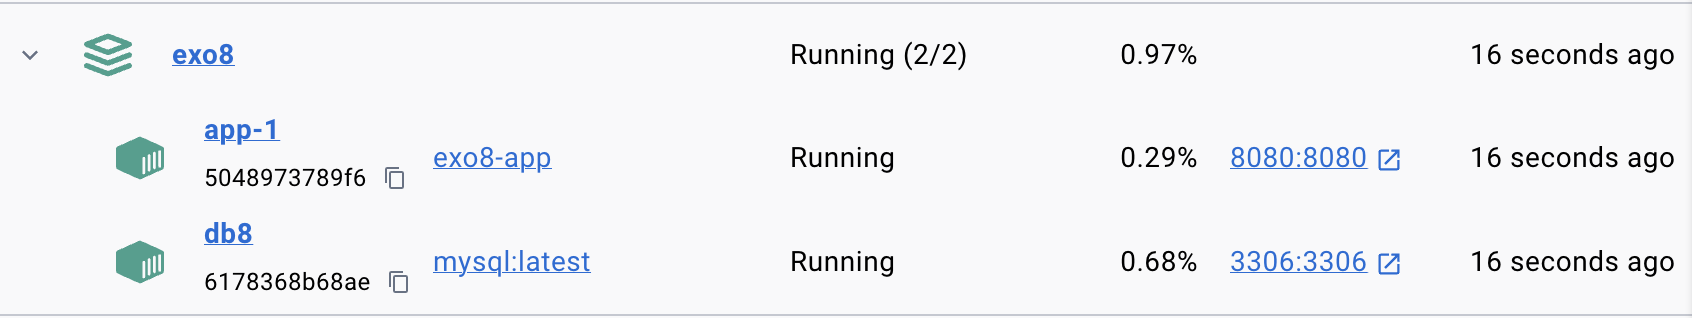
\includegraphics[width=\textwidth]{images/exo8_desktop.png}
    \caption{Les services lancés sur Docker Desktop}
    \label{fig:exo8_services}
\end{figure}

\begin{figure}[hbtp]
    \centering
    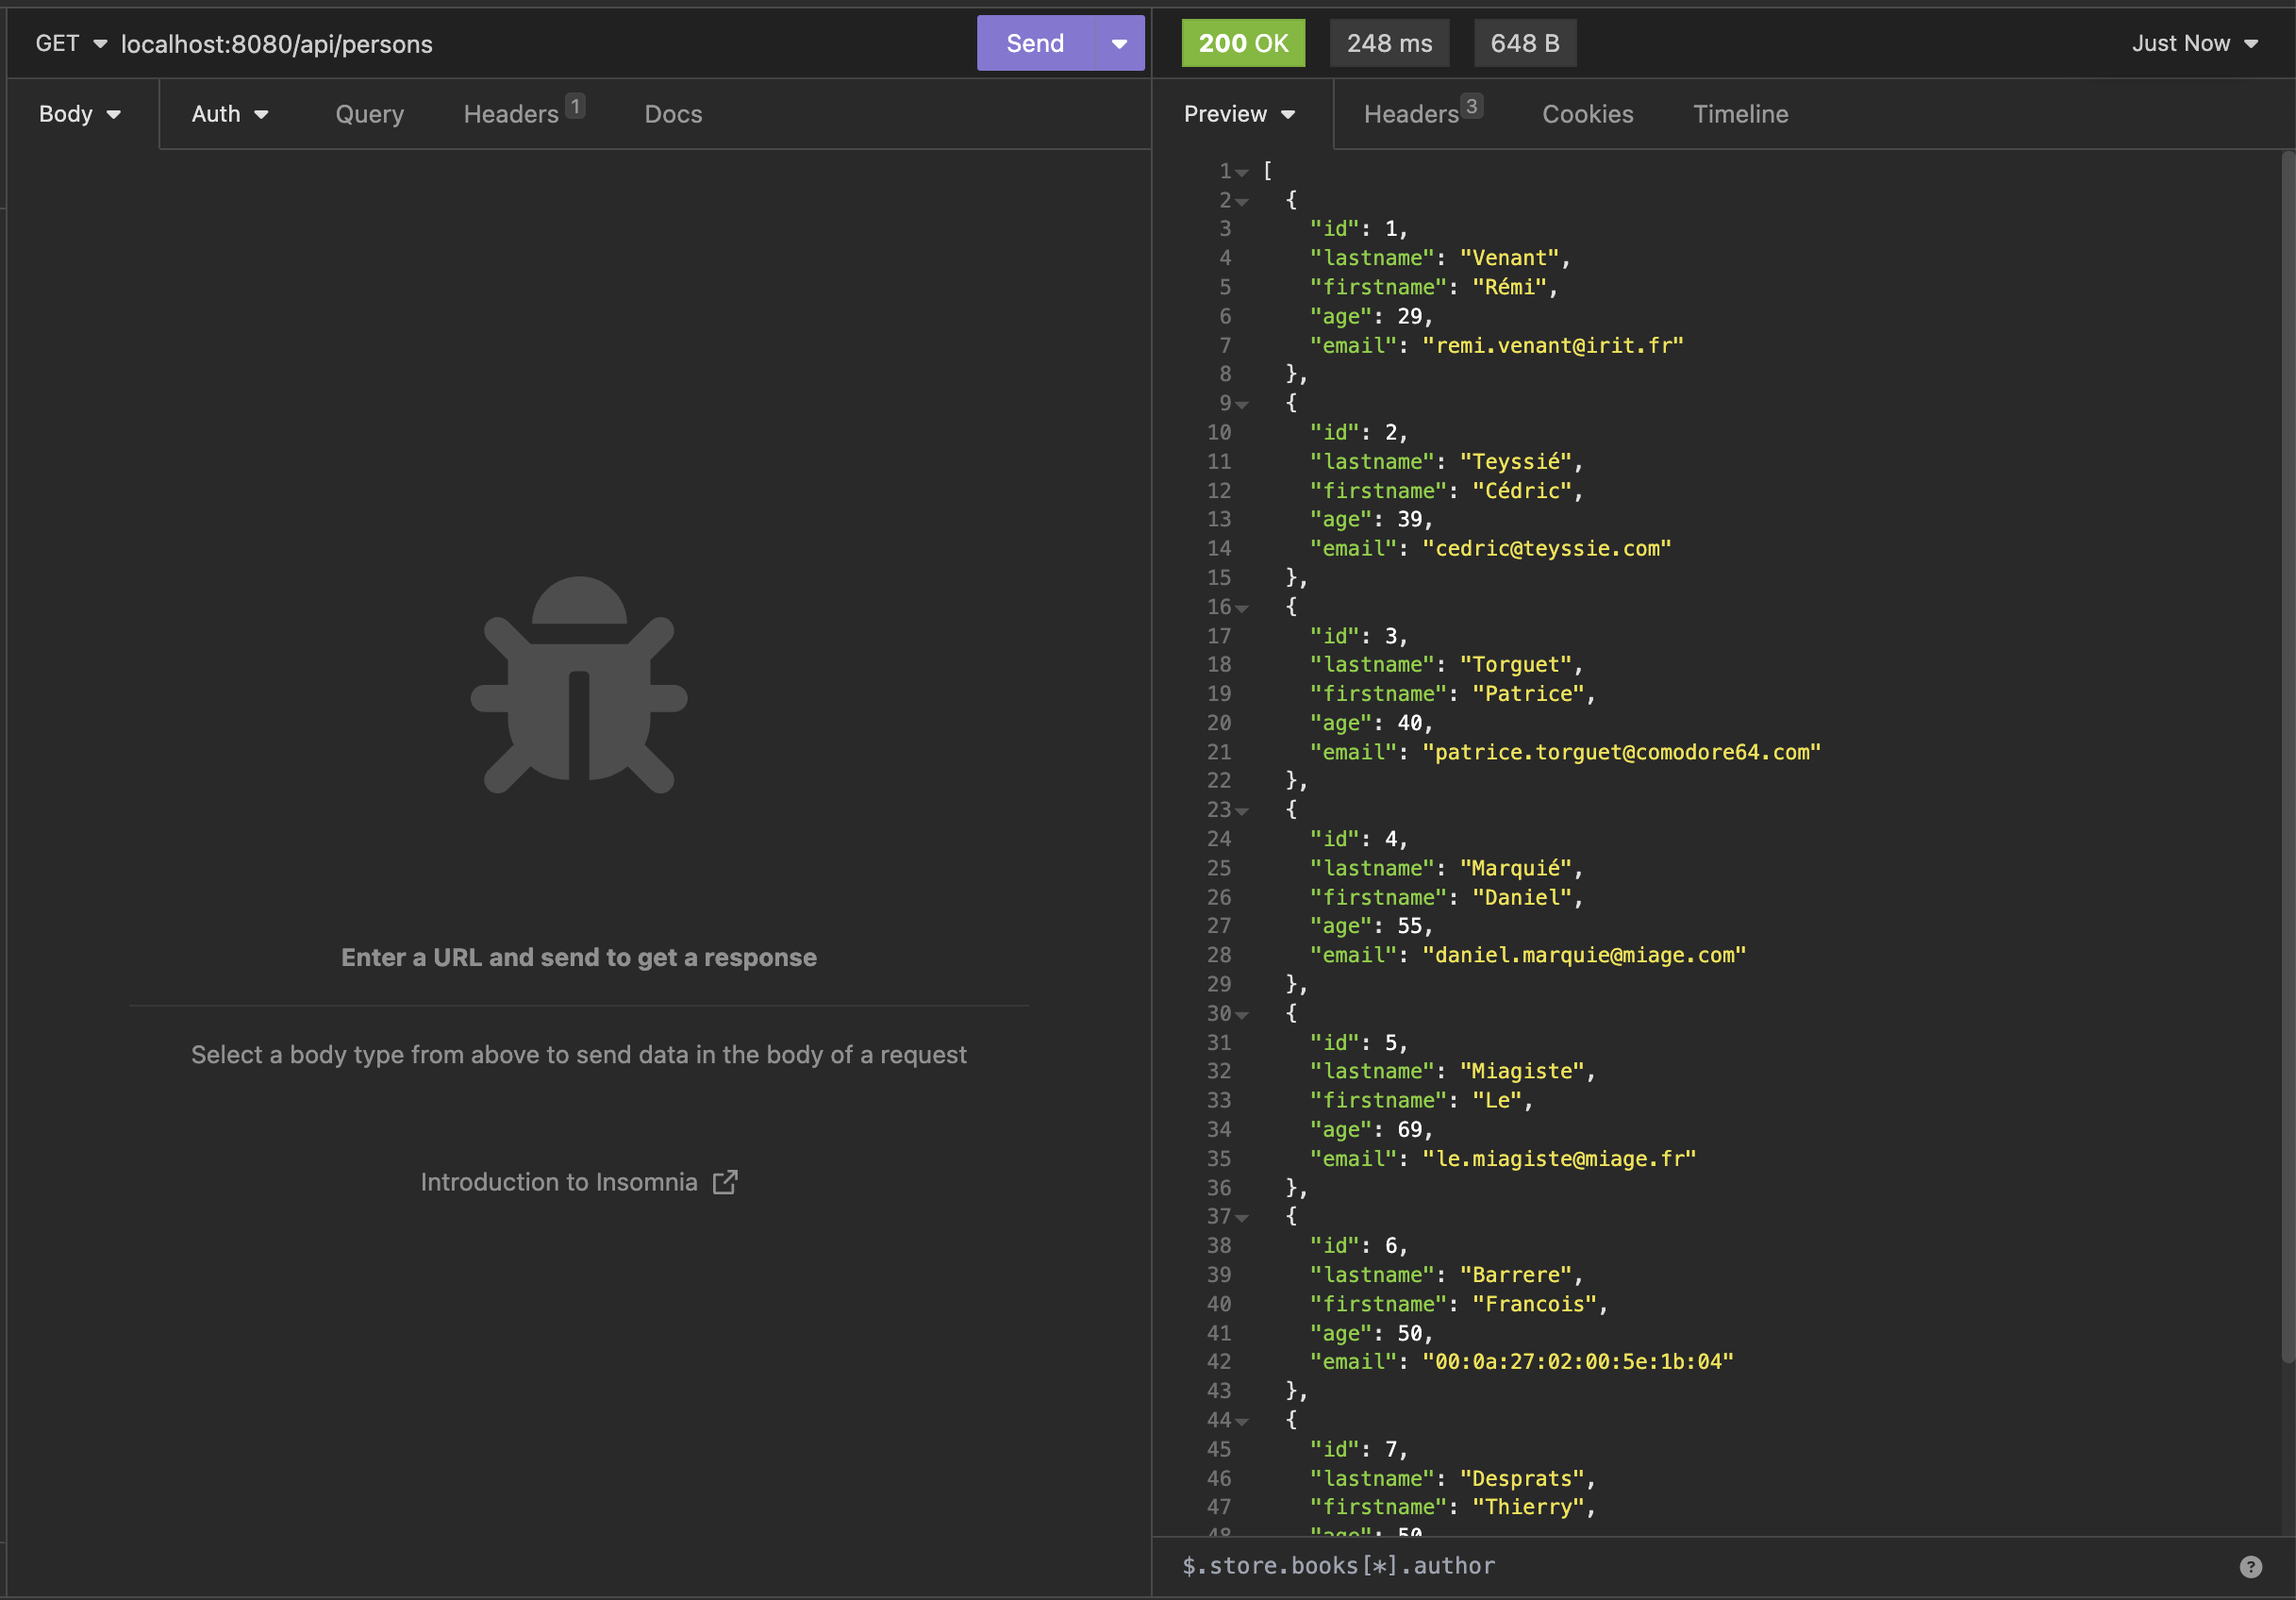
\includegraphics[width=\textwidth]{images/exo8_api.png}
    \caption{Test de l'app Spring Boot et de la BDD pour l'exercice 8}
    \label{fig:exo8_api}
\end{figure}

\subsubsection*{Sources}
Dockerfile :
\begin{verbatim}
# FIRST VERSION WITH BUILD
# FROM maven:3.9.5-eclipse-temurin-21 AS builder
# 
# WORKDIR /app
# 
# COPY pom.xml .
# COPY src ./src
# 
# RUN mvn clean install
# 
# FROM maven:3.9.5-eclipse-temurin-21 AS runner
# 
# WORKDIR /app
# 
# COPY --from=builder /app/target/*.jar ./app.jar
# 
# ENTRYPOINT ["java", "-jar", "app.jar"]

# SECOND VERSION WITHOUT BUILD
FROM maven:3.9.5-eclipse-temurin-21 AS runner

WORKDIR /app

COPY target/devops-1.0.jar ./app.jar

CMD ["java", "-jar", "app.jar"]
\end{verbatim}
\hrule
\vspace{0.4cm}
docker-compose.yml :
\begin{verbatim}
version: '3'

services:
    db8:
        image: mysql:latest
        container_name: db8
        volumes:
            - db_data:/var/lib/mysql
            - ./data.sql:/docker-entrypoint-initdb.d/init.sql
        environment:
            MYSQL_USER: dev
            MYSQL_DATABASE: test
            MYSQL_ROOT_PASSWORD: root
            MYSQL_PASSWORD: root
        ports:
            - "3306:3306"

    app:
        build: .
        ports:
            - "8080:8080"
        depends_on:
            - db8

    volumes:
        db_data:
\end{verbatim}

\newpage

\subsection*{Exercice IX}
\begin{figure}[hbtp]
    \centering
    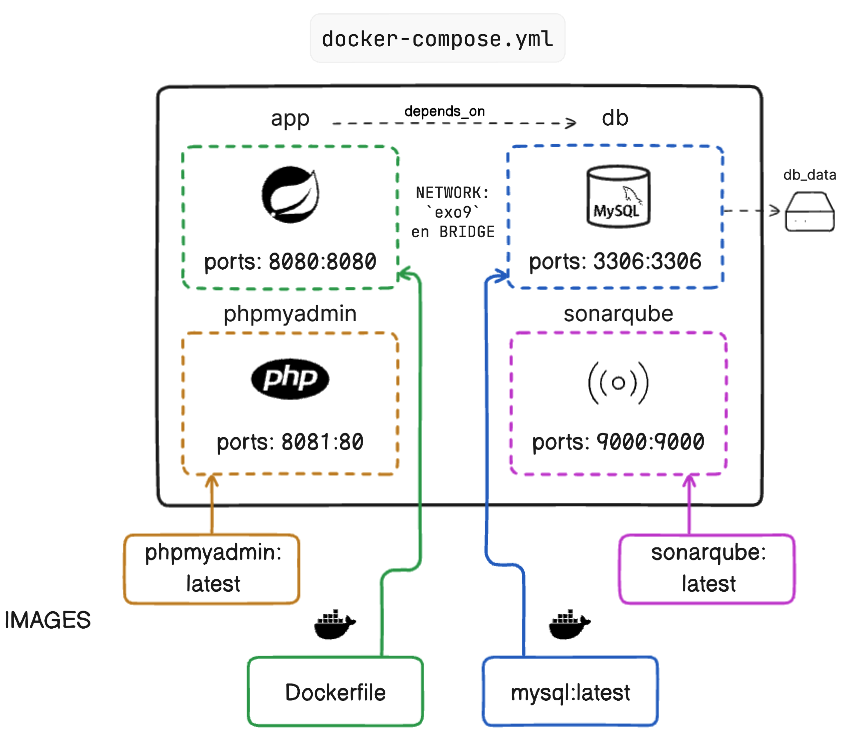
\includegraphics[width=\textwidth]{images/exo9.png}
    \caption{Architecture de l'exercice IX}
    \label{fig:exo9}
\end{figure}
\subsubsection*{Commandes}
Commandes à réaliser :
    
\begin{verbatim}
    docker compose up -d
\end{verbatim}
Pour arrêter et supprimer les containers, vous pouvez utiliser :

\begin{verbatim}
    docker compose down
\end{verbatim}
Vous pouvez retrouver les différents services sur les liens suivants :
\begin{itemize}
    \item \href{http://localhost:8080}{http://localhost:8080} pour l'application Spring Boot
    \item \href{http://localhost:8081}{http://localhost:8081} pour phpMyAdmin
    \item \href{http://localhost:9000}{http://localhost:9000} pour 
    Sonarqube
\end{itemize}
Pour utiliser sonarqube, il faut créer un projet et générer un token. Ce token est à renseigner dans le projet Spring Boot si l'on souhaite que Sonarqube soit actualisé à chaque build. Dans mon cas, l'analyse peut être lancée grâce à la commande suivante :
\begin{verbatim}
mvn clean verify sonar:sonar \
    -Dsonar.projectKey=PROJECT_KEY \
    -Dsonar.projectName='PROJECT_NAME' \
    -Dsonar.host.url=http://localhost:9000 \
    -Dsonar.token=YOUR_TOKEN \
\end{verbatim}

\subsubsection*{Résultats}
\begin{figure}[hbtp]
    \centering
    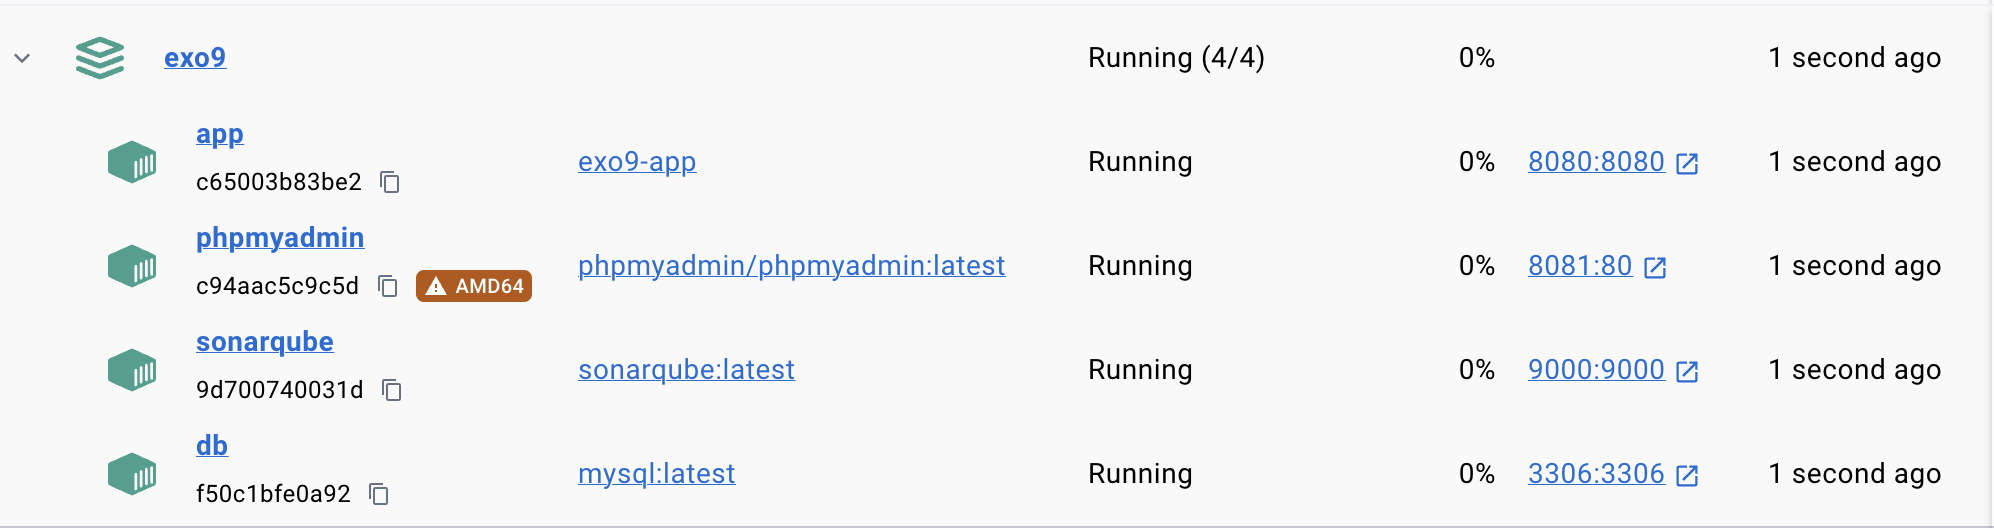
\includegraphics[width=\textwidth]{images/exo9_desktop.png}
    \caption{Les services lancés sur Docker Desktop}
    \label{fig:exo9_services}
\end{figure}

\begin{figure}[hbtp]
    \centering
    \includegraphics[width=\textwidth]{images/phpMyAdmin.png}
    \caption{Interface phpMyAdmin avec la table `personnes'}
    \label{fig:phpmyadmin}
\end{figure}

\begin{figure}[hbtp]
    \centering
    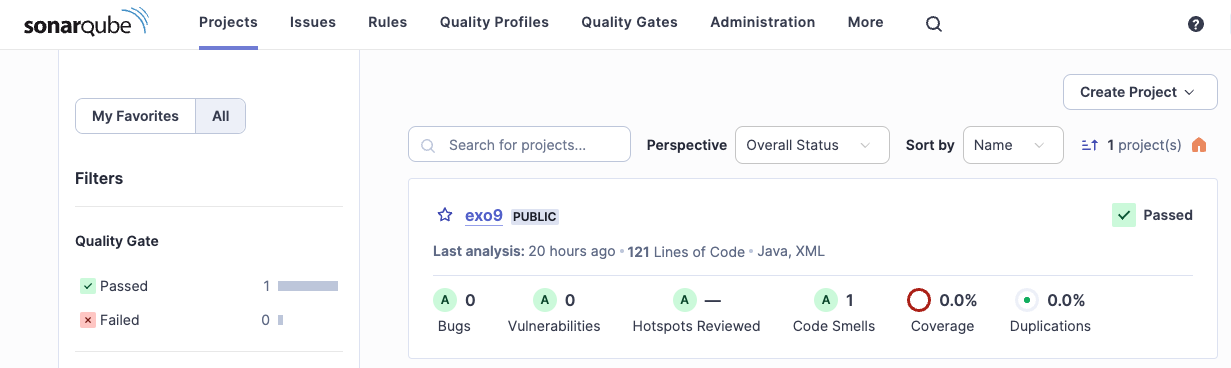
\includegraphics[width=\textwidth]{images/sonarqube.png}
    \caption{Interface Sonarqube}
    \label{fig:Sonarqube}
\end{figure}

\begin{figure}[hbtp]
    \centering
    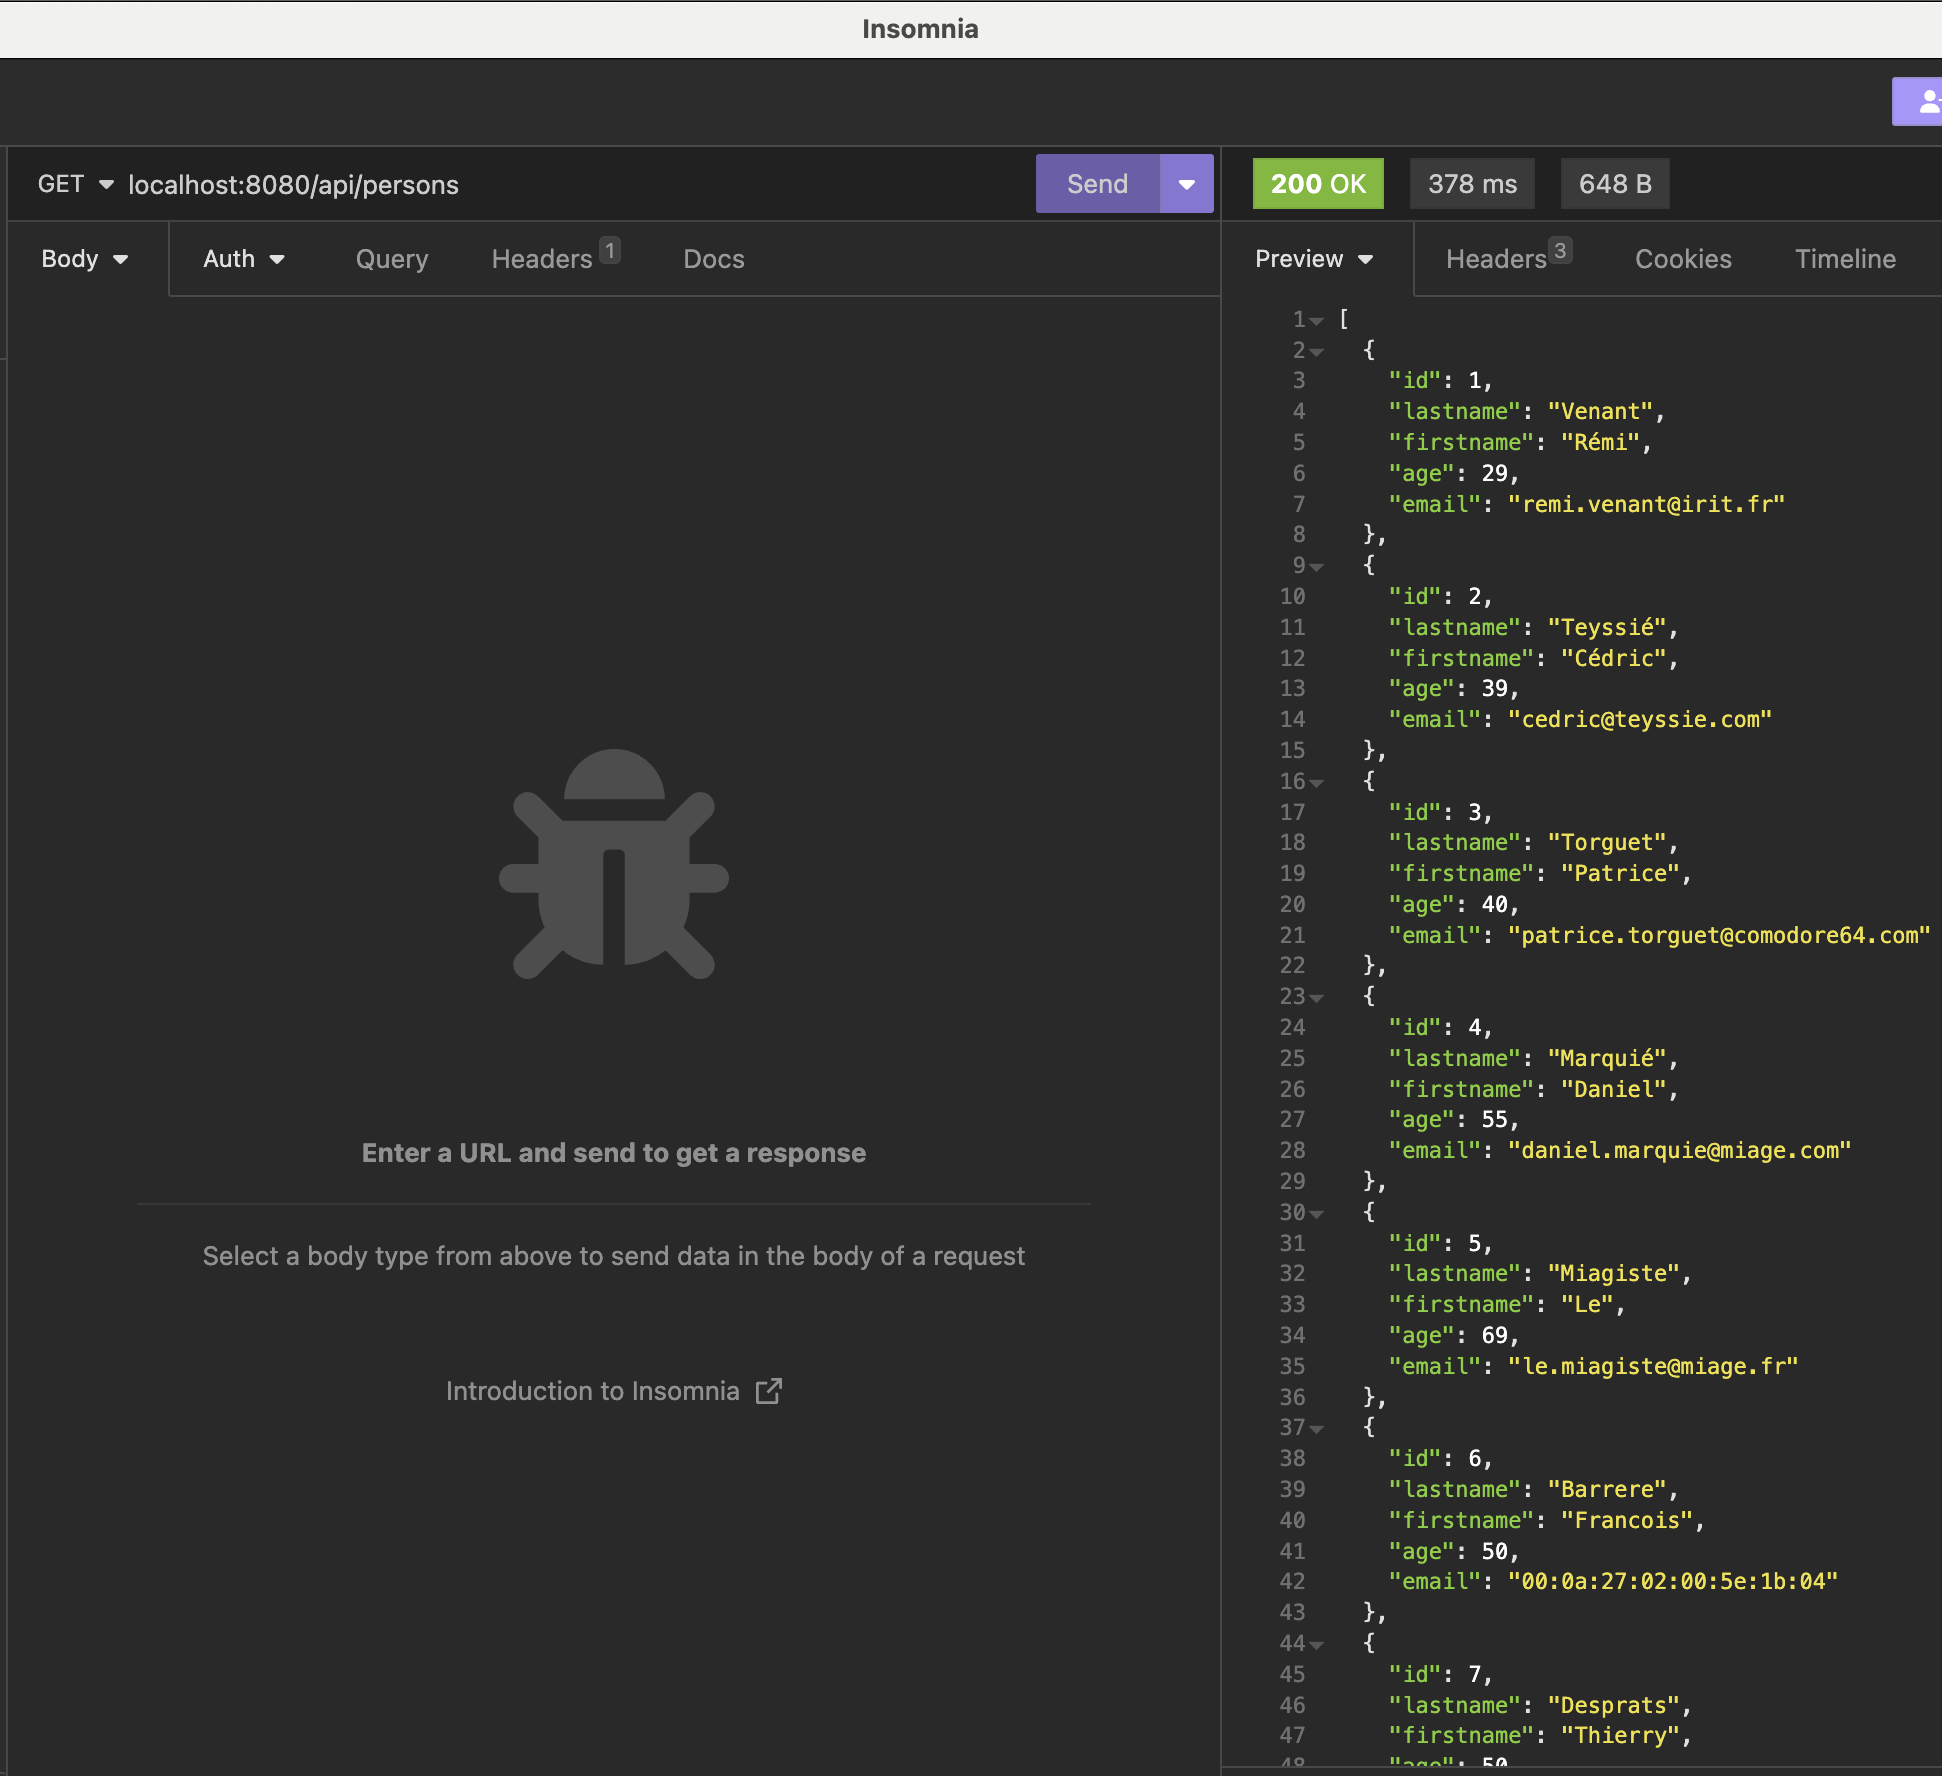
\includegraphics[width=\textwidth]{images/exo9_api.png}
    \caption{Test de l'app Spring Boot et de la BDD pour l'exercice 9}
    \label{fig:exo9_api}
\end{figure}

\newpage

\subsubsection*{Sources}
Dockerfile :
\begin{verbatim}
FROM maven:3.9.5-eclipse-temurin-21 AS builder

WORKDIR /app

COPY target/devops-1.0.jar ./app.jar

CMD ["java", "-jar", "app.jar"]
\end{verbatim}
\hrule
\vspace{0.4cm}
docker-compose.yml :
\begin{verbatim}
version: '3'

services:
    db:
        image: mysql:latest
        container_name: db
        volumes:
            - db_data:/var/lib/mysql
            - ./data.sql:/docker-entrypoint-initdb.d/init.sql
        environment:
            MYSQL_USER: dev
            MYSQL_DATABASE: test
            MYSQL_ROOT_PASSWORD: root
            MYSQL_PASSWORD: root
        ports:
            - "3306:3306"
        networks:
            - exo9

    app:
        build: .
        container_name: app
        ports:
            - "8080:8080"
        depends_on:
            - db
        networks:
            - exo9

    sonarqube:
        image: sonarqube:latest
        container_name: sonarqube
        ports:
            - "9000:9000"
        environment:
            - SONARQUBE_JDBC_URL=jdbc:mysql://db:3306/sonarqube
            ?useUnicode=true
            &characterEncoding=utf8
            &rewriteBatchedStatements=true
            &useConfigs=maxPerformance
            &useSSL=false
            - SONARQUBE_JDBC_USERNAME=dev
            - SONARQUBE_JDBC_PASSWORD=root
        networks:
            - exo9

    phpmyadmin:
        image: phpmyadmin/phpmyadmin:latest
        container_name: phpmyadmin
        environment:
            - PMA_ARBITRARY=1
            - PMA_HOST=db
            - PMA_PORT=3306
        ports:
            - "8081:80"
        networks:
            - exo9

    networks:
        exo9:
            driver: bridge

    volumes:
        db_data:
    
\end{verbatim}

